%!TEX root = ../paper.tex

\subsection{Classification}
\label{sec:classification}

% TODO: Features sind die gleichen wie beim Clustering!

After we calculate the clusters and their labels for all blog posts in a database, we need a method to classify new blog posts.
Without such a method, we would have to re-run the clustering algorithm on the entire dataset every time a new post should be clustered.
To achieve this we calculate the same features vectors for the single new blog post, as we did for the blog posts in the original clustering.
Based on these feature vectors we can now decide to which cluster the blog post belongs.


The first naive idea that came into our mind was to calculate the euclidean distance from the blog post to the central points of each cluster.
The resulting cluster would then be the one with the lowest distance.
While this method is computationally simple and fast, it might not provide the best possible results.
Therefore we looked at more sophisticated approaches that were used for similar problems before.
We applied two of those methods, a k-Nearest neighbor algorithm~\cite{peterson2009k} and a Support Vector Machine~\cite{kolari2006svms}.


\subsubsection{k-Nearest Neighbor}
\label{sec:k_nearest_neighbor}


The k-Nearest Neighbor algorithm selects the $k$ vectors which are closest to the feature vector of the new blog post.
Then it returns the cluster that is prevalent amongst these neighbors as a result.
For example consider the scenario depicted in Figure~\ref{fig:naive}.
The naive method of calculating the euclidean distance between the cluster center and the feature vector of the new blog post would have cluster 1 as a result.
However the k-Nearest Neighbor algorithm with, for example $k=5$, returns cluster 2, because four out of the five closest neighbors belong to cluster 2.
Intuitively, this appears like the better solution because the feature vector of the new blog post seems to be naturally belonging to cluster two.


\begin{figure}[h]
    \centering
    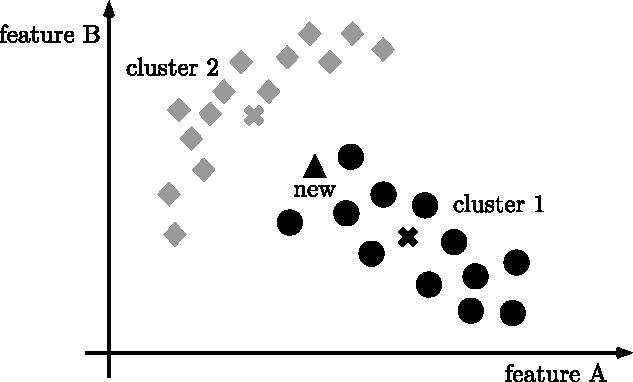
\includegraphics[width=0.6\textwidth]{images/naive.pdf}
    \caption{The naive approach, which calculates the euclidean distance to the center of the cluster, would put the new blog post into cluster 1. The k-Nearest Neighbor algorithm would return cluster 2 as a result.}
    \label{fig:naive}
\end{figure}


\subsubsection{Support Vector Machine}
\label{sec:support_vector_machine}


A Support Vector Machine creates a model to distinguish between the different clusters by calculating borders between them.
These borders can be thought of as functions in the same vector space as the feature vectors.
If the Support Vector Machine uses a linear model, this might look like Figure~\ref{fig:svm}, represented in a two-dimensional graph.
Both, the dotted and the dashed line serve as examples for a possible border, but the Support Vector Machine should usually tend to use the model with more distance to all feature vectors.
In this case, the dashed line would more accurately divide cluster 1 and 2.


\begin{figure}[h]
    \centering
    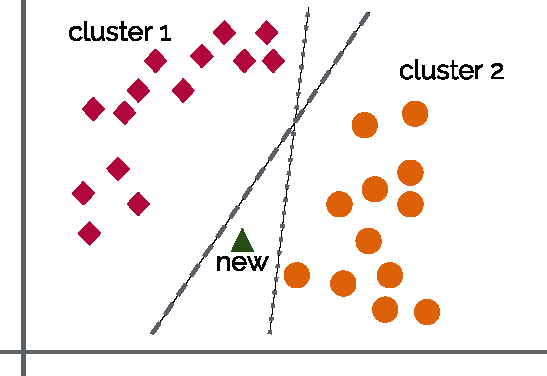
\includegraphics[width=0.6\textwidth]{images/svm.pdf}
    \caption{Two differently configured Support Vector Machines might provide the two different lines as borders between the different clusters. The dotted line would result in the blog post belonging to cluster 1, while the dashed line would return cluster 2 as a result.}
    \label{fig:svm}
\end{figure}
